\section{Module Functions and Integration}
\label{sec:modules}
Section~\ref{sec:design} defines the architecture and shared dispatch
contract. This section specifies the runtime context passed to adapters and
the route-specific admission, approval, and evidence steps.

\subsection{Task, Harness, and Context}
Task and chat entry points create or join a workspace channel. The task
runtime manages membership, roles, task state, and shared execution context;
a harness registry adapts agent engines to a common execution interface. This
separation lets agents collaborate through shared tasks and channel resources
without coupling their engine-specific turn protocol to a production scene.
At each turn, the prompt builder assembles the task, active scene description,
line--product--recipe--run state, channel profile, agent binding, and retrieved
memory. The resulting context supports process-aware proposals, while the
dispatcher independently checks authority and the operation handler resolves
current state before a write.

Direct REST and selected stdio-MCP operation calls reach the same dispatcher
without a task or harness turn. REST authentication and identity resolution
follow Section~\ref{sec:executionflow}; each handler reads live route state
at invocation. Handlers receive the resolved actor, channel, and operation
arguments through the same interface for either entry route; records are keyed
by the identifiers supplied in each request. A registered task additionally
receives prompt context and a scoped tool catalog. Catalog visibility alone
does not grant write authority: the dispatcher checks authority at invocation.

\subsection{Shared Dispatch and Device Admission}
\label{sec:governed}
Each operation must satisfy the predicates in
Eq.~(\ref{eq:dispatch-contract}) before handler selection; the selected
handler then revalidates route-specific state. Scene configuration maps
semantic signals and controls to
drivers and specifies process objectives and guards. Capability profiles and
tool policies narrow available operations, while resource bindings constrain
accessible nodes, controls, and recipes. Optional data-acquisition (DAQ),
manufacturing execution system (MES), analysis, retrieval, optimization, and
digital-twin services are invoked through registered handlers. The application supplies its optimization strategy;
the framework coordinates context, operation access, and execution.

The target band describes a desired process outcome. It is not the admissible
write interval: the latter is computed from engineering, product, recipe, and
route-specific limits below. A candidate can satisfy every write constraint
while the measured process value remains outside its target band.

Actuator writes converge on the shared device-write admission point.
For an online node write, the admissible value interval is
\begin{equation}
\mathcal{I}^{\mathrm{online}}_n(t)=
\mathcal{H}_n\cap\mathcal{L}^{\mathrm{base}}_n\cap\mathcal{L}^{\mathrm{prod}}_n(t)\cap\mathcal{L}^{\mathrm{rec}}_n(t),
\label{eq:admission}
\end{equation}
where $\mathcal{H}_n$ is the hard engineering range and
$\mathcal{L}^{\mathrm{base}}_n$, $\mathcal{L}^{\mathrm{prod}}_n$, and
$\mathcal{L}^{\mathrm{rec}}_n$ are the baseline, active-product, and
active-recipe limits; the $\mathcal{L}$ limits here are deliberately named
apart from the policy and binding predicates of
(\ref{eq:dispatch-contract}). Missing optional limits impose no
restriction; an empty intersection rejects the request and identifies the
excluding layer. Recipe dispatch validates the replacement recipe against
the hard, baseline, and product limits rather than the previous recipe
window. Step, interval, and hold-window checks apply as configured for each route.
These application-level checks bound commands alongside independent
programmable-logic-controller and safety-instrumented protection. They do not
replace equipment interlocks or certify the safety of a plant deployment.

\subsection{Approval, Execution, and Evidence}
\label{sec:routes}
\label{sec:mech}
\label{sec:objective}
\label{sec:nodeexec}
\label{sec:ack}
\label{sec:agentloop}
Routes add timing checks and, when required by operation and configuration,
approval checks. Outside benchmark mode, online agent and manual node writes
enforce a 60\,s minimum interval between successful writes. Recipe trials use
a per-line cadence (300\,s by default), and recipe intervals are anchored to approval.
Manual approval binds an actor and proposed operation to candidate values,
applicable limits, expiry, and the active line--product--recipe--run tuple.
After approval, the handler rechecks authority and compares the current tuple
with the approved tuple before entering device-write dispatch. Single-parameter waits
expire after 180\,s by default; recipe-dispatch approvals use a 30-minute
window. A changed recipe definition requires a new
\texttt{recipe\_apply} proposal.

Fig.~\ref{fig:hitl}(a) illustrates the four-layer interval in
Eq.~(\ref{eq:admission}) as a conceptual intersection of configured bounds;
its horizontal positions do not represent measured or run-derived values.
Panel (b) shows the decision and rechecks when approval is required.

\begin{figure*}[!t]
\centering
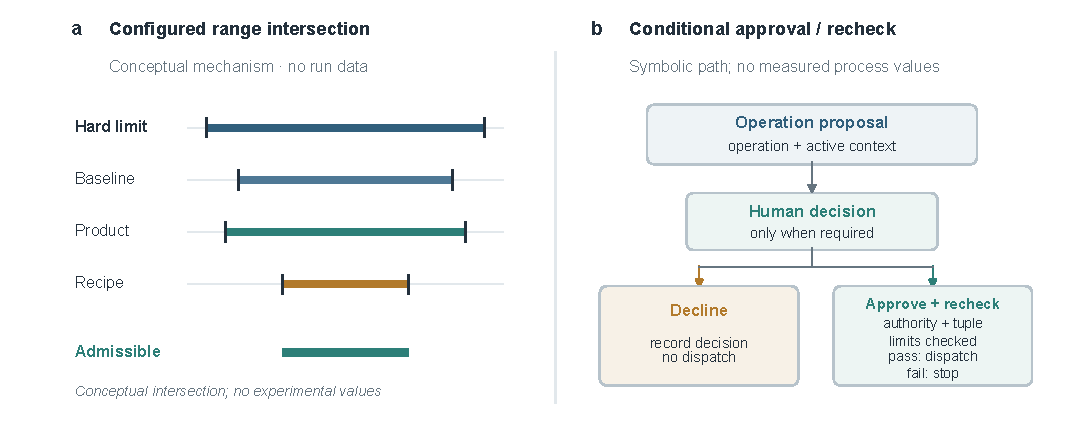
\includegraphics[width=\textwidth]{resources/fig5-nature-A.pdf}
\caption{Admission and approval boundaries. (a) Conceptual intersection of
the hard, baseline, product, and recipe bounds in Eq.~(\ref{eq:admission});
horizontal positions are schematic and encode no experimental values.
(b) When approval is required, a decline prevents dispatch; approval is
followed by authority, context, and limit rechecks.}
\label{fig:hitl}
\end{figure*}

A \texttt{recipe\_trial} illustrates the operation sequence: the handler
checks the bound recipe, active run, candidate parameters, and route timing;
if required, it requests approval; after revalidation, it submits a bounded
batch through the configured driver and returns a per-parameter receipt.
The caller can obtain later DAQ observations separately and may then update,
apply, or roll back a recipe. A trial neither saves nor applies a recipe
version. The driver registry maps semantic controls to configured protocol
drivers, keeping protocol details out of agent operation arguments.

At dispatch, the handler resolves the active production context, intersects
the applicable bounds, and applies route timing and approval requirements
before invoking the configured driver. The driver returns a graded receipt;
later acquisition samples are stored separately and linked to the operation
when the route provides matching context and timestamps. The evaluation uses
deterministic tool invocation and does not assess operator performance.

Receipts and observations answer different questions. A command result is
graded as readback-verified, transport-acknowledged, or unverified; a
readback mismatch can trigger up to three reads at 2\,s intervals. Recipe
batches retain per-parameter verification outcomes. A readback-verified result
records that the returned value matched the request; a transport acknowledgement
alone does not establish that the device applied it, and an unverified result
does not establish a matching readback. DAQ stores subsequent timestamped
process observations, while recipe history, approvals, and task records remain
with their owning services. Identifiers and timestamps can link these records
when available, but a later observation alone does not prove that the command
caused the measured change. Section~\ref{sec:eval} evaluates selected parts of
this evidence chain under the stated test conditions.

